\section{Paredes y agujeros}
A pesar de la aparente simplicidad de una pared, la alta configurabilidad que pretendemos ofrecer con nuestro software hace que la complejidad se dispare. No es suficiente con poder crear una pared satisfactoriamente, tenemos que hacerlo para todos los tamaños y orientaciones posibles. Además, otro requerimiento es el de poder introducir puertas y ventanas en una pared, y para ello se requiere que la pared tenga un hueco, y eso aumenta considerablemente la complejidad de la geometría de la pared.

En este apartado voy a describir el proceso de desarrollo de las paredes en 2 iteraciones, una primera en la que creamos una estructura básica para las paredes, y otra en la que tenemos en cuenta las ventanas y puertas.

%%%%%%%%%%%%%%%%%%%%%%%%%%%%%%%%%%%%%%%%%%%%%%%%%%%%%%%%%%%%%%%%%%%%%%%%%%%%%
%%%%%%%%%%%%%%%%%%%%%%%%%%%%%%%%%%%%%%%%%%%%%%%%%%%%%%%%%%%%%%%%%%%%%%%%%%%%%
%%%%%%%%%%%%%%%%%%%%%%%%%%%%%%%%%%%%%%%%%%%%%%%%%%%%%%%%%%%%%%%%%%%%%%%%%%%%%
\subsection{Generación de la estructura básica de la pared}
\label{subsec:gen1}
El primer paso ha sido crear una definición de los datos que recibiremos para describir cómo ha de ser la pared. Básicamente se trata de una lista de puntos en dos dimensiones y un valor booleano que indica si esta lista debe cerrarse conectando el último punto con el primero. Esto último es importante porque, como veremos a continuación, la geometría de una esquina ``suelta" es diferente a la de una esquina que conecta dos paredes entre sí (Fig. \ref{fig:vertical_view_walls}).

\begin{figure}[h]
    \centering
    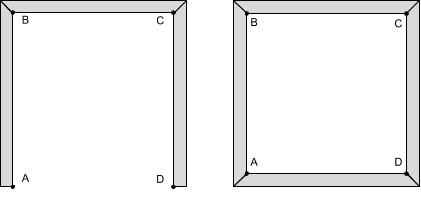
\includegraphics[width=0.65\linewidth]{Vista_Vertical_Paredes}
    \caption{Paredes en vista vertical.}
    \label{fig:vertical_view_walls}
\end{figure}

De este modo como podemos imaginar estos datos nos permiten no sólo crear habitaciones sino también paredes únicas o incluso otros tipos de estructuras, normalmente interiores, similares a una pared. La intención es que en el futuro este software pueda utilizarse en otras herramientas para hacer diseños más complicados como el plano de una planta completa de un edificio.

Así pues, en la figura \ref{fig:io_generatewalls} se puede ver la conversión de los datos que esperamos conseguir:

\begin{figure}[H]
    \centering
    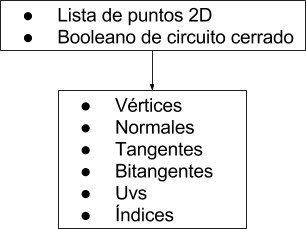
\includegraphics[scale=0.45]{IO_paredes}
    \caption{Input y output de GenerateWalls.}
    \label{fig:io_generatewalls}
\end{figure}

Nótese que el output está formado por listas de valores planos porque el motor así lo requiere. Por ejemplo, la lista de vértices está formada por los valores ``x,y,z" de cada uno  sucesivamente.

La parte más sencilla en el momento de generar una pared es encontrar las posiciones de los diferentes vértices que van a formarla. Por cada pared tenemos tres puntos 2D relevantes: las esquinas izquierda de las paredes anterior, actual, y siguiente. A partir de estos tres puntos podemos deducir la información de la figura \ref{fig:wall_vectors}, donde los vectores N1 y N2 son las normales de cada pared, siempre hacia la izquierda.

\begin{figure}[H]
    \centering
    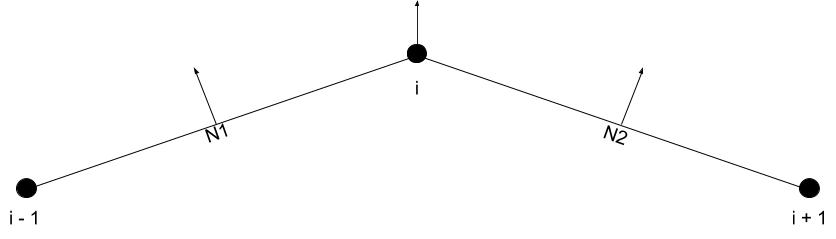
\includegraphics[width=\linewidth]{data_from_3_points}
    \caption{Vectores extraídos a partir de 3 puntos consecutivos.}
    \label{fig:wall_vectors}
\end{figure}

N1 y N2 pueden obtenerse fácilmente normalizando los vectores de un punto a otro, y girándolos:

\begin{lstlisting}
glm::vec3 v_pc = current - previous;
glm::vec3 v_cn = next - current;

glm::vec3 current_normal = glm::normalize(glm::vec3(-v_cn.z, 0.0f, v_cn.x));
glm::vec3 previous_normal = glm::normalize(glm::vec3(-v_pc.z, 0.0f, v_pc.x));
\end{lstlisting}

El vector que hay sobre la esquina ``i" representa la dirección que ha de seguir la línea que separa ambas paredes y se obtiene como la suma y normalización de los vectores N1 y N2:

\begin{lstlisting}
glm::vec3 dir = glm::normalize(current_normal + previous_normal);
\end{lstlisting}

Por último debemos tener en cuenta el grosor que se espera que tenga la pared, dado que si avanzáramos siempre la misma distancia en el vector director el grosor de estas dependería del ángulo que formen con sus paredes adyacentes. Esto se resuelve con trigonometría:

\begin{lstlisting}
dir *= wall_depth / abs(glm::dot(current_normal, dir));
\end{lstlisting}

Recordemos que el producto punto de dos vectores normales es el coseno del ángulo que forman entre sí. En este momento ``dir" incluye la dirección y distancia entre nuestro punto ``i" y la esquina, y ya podemos obtener dichos puntos y guardarlos para procesarlos posteriormente.

En el caso de que la pared que estamos generando no haga esquina con otra, generaremos dichos puntos simplemente usando los vectores normales de cada pared, lo cual es mucho más sencillo:

\begin{lstlisting}
dir = wall_depth * current_normal;
\end{lstlisting}

Una limitación de este sistema es que los puntos deben introducirse en sentido anti-horario respecto al interior de la habitación. De lo contrario la normal de cada pared queda invertida y estas se extienden hacia el lado opuesto al que deberían, provocando algunos artefactos no deseados.

%%%%%%%%%%%%%%%%%%%%%%%%%%%%%%%%%%%%%%%%%%%%%%%%%%%%%%%%%%%%%%%%%%%%%%%%%%%%%
%%%%%%%%%%%%%%%%%%%%%%%%%%%%%%%%%%%%%%%%%%%%%%%%%%%%%%%%%%%%%%%%%%%%%%%%%%%%%
%%%%%%%%%%%%%%%%%%%%%%%%%%%%%%%%%%%%%%%%%%%%%%%%%%%%%%%%%%%%%%%%%%%%%%%%%%%%%
\subsection{Índices para la estructura básica}
Para referirnos a cada uno de los vertices usaremos la nomenclatura ``A, B, A2, B2" como puede verse en la figura \ref{fig:nomenclatura_vertices}, además de los correspondientes ``AH, BH, A2H, B2H" en la parte alta de la pared. Posteriormente, para conectar los vértices generados nos basamos en la estructura de un cubo como se ve en la figura \ref{fig:estructura_cubo}.

\begin{figure}[H]
    \centering
    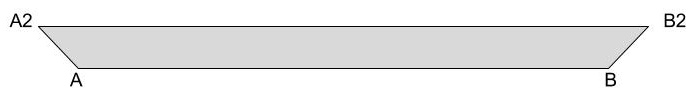
\includegraphics[width=0.75\linewidth]{Nomenclaturas_vertices}
    \caption{Nomenclatura básica de los vértices.}
    \label{fig:nomenclatura_vertices}
\end{figure}

\begin{figure}[H]
	\centering
	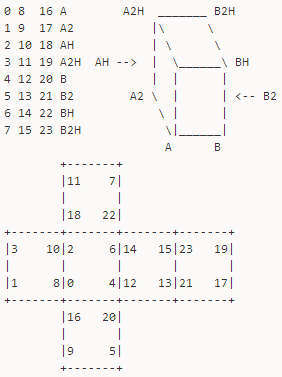
\includegraphics[scale=0.75]{Cube_structure}
	\caption{Estructura de un cubo.}
	\label{fig:estructura_cubo}
\end{figure}

Lo primero que podemos ver es que hay 23 vértices y no 8 como cabría esperar. Esto se debe a que en el momento de renderizar, se interpola la normal de cada vértice con la de sus vecinos; si el mismo vértice se encuentra en dos caras distintas, la normal del vértice no coincide con la de la superficie en la cara que estamos pintando. El resultado de esto sería que el color varía en los bordes de cada cara. Esta propiedad es muy útil para objetos que no tienen ángulos tan marcados, pero en nuestro caso queremos que las caras sean muy marcadas y totalmente planas.

Para solucionarlo repetimos cada vértice tantas veces como el número de caras en el que se encuentre, de modo que aunque todos se encuentren en la misma posición, cada cara está utilizando un vértice distinto. Los índices se definen en grupos de 3 vértices del siguiente modo, teniendo en cuenta la numeración de la anterior imagen:

\begin{lstlisting}
#define INDICES {\
    12, 13, 15,     15, 14, 12,     21, 17, 19, \
    19, 23, 21,     1,  8,  10,     10, 3,  1,  \
    0,  4,  6,      6,  2,  0,      5,  20, 16, \
    16, 9,  5,      11, 18, 22,     22, 7,  11, \
}
\end{lstlisting}

Para definirlos se ha tenido especial cuidado en el orden de estos, pues la dirección de las normales dependen de dicho orden.

%%%%%%%%%%%%%%%%%%%%%%%%%%%%%%%%%%%%%%%%%%%%%%%%%%%%%%%%%%%%%%%%%%%%%%%%%%%%%
%%%%%%%%%%%%%%%%%%%%%%%%%%%%%%%%%%%%%%%%%%%%%%%%%%%%%%%%%%%%%%%%%%%%%%%%%%%%%
%%%%%%%%%%%%%%%%%%%%%%%%%%%%%%%%%%%%%%%%%%%%%%%%%%%%%%%%%%%%%%%%%%%%%%%%%%%%%
\subsection{Modificando la estructura para permitir la inclusión de ventanas}
\label{subsec:gen2}
Una vez ya tenemos los primeros resultados debemos implementar la posibilidad de añadir puertas y ventanas a la habitación. Insertar el modelo correspondiente en cada caso no será un problema, pero para que el efecto sea convincente debemos poder ver a través de estos. Eso implica que tendremos que modificar la geometría de las paredes para que incluya huecos donde tengan que ir dichas ventanas y puertas.

Igual que como hemos hecho con las paredes inicialmente, vamos a definir el input: por cada hueco tendremos un punto 3D (que como veremos a continuación, no necesariamente debe colisionar con una pared), una altura y un ancho. El input/output del algoritmo completo para generar paredes quedaría así como se puede ver en la figura \ref{fig:io_generatewindows}

\begin{figure}[H]
    \centering
    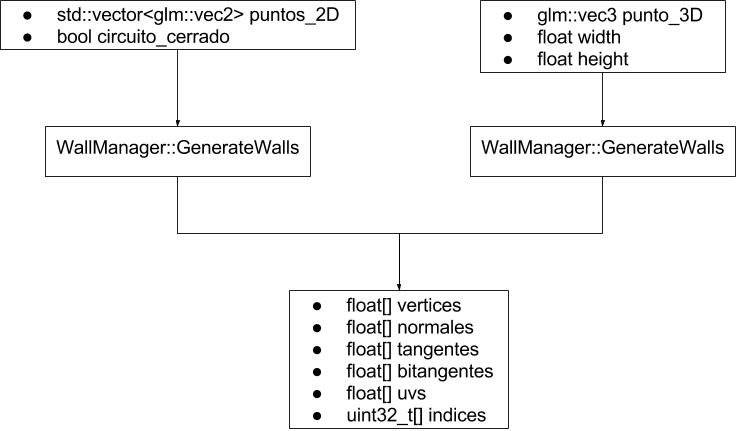
\includegraphics[width=0.75\linewidth]{I_O_ventanas}
    \caption{Nuevo input y output de GenerateWalls, incluyendo ventanas.}
    \label{fig:io_generatewindows}
\end{figure}

Para empezar tenemos que adaptar las paredes que ya hemos generado. Nos interesa que la generación de ventanas se limite a trabajar sobre un solo plano, de modo que eliminaremos los planos anterior y posterior de la pared para añadirlos después con la nueva geometría. Aunque intuitivamente parezca que esto supone simplificar la geometría de lo que hemos hecho hasta ahora, en realidad la vamos a complicar un tanto. Es fácil darse cuenta de que los planos anterior y posterior de la pared van a ser siempre idénticos, pero el plano posterior es algo más alargado debido a la geometría de las esquinas que hemos visto en el apartado \ref{subsec:gen1}.

\begin{figure}[H]
    \centering
    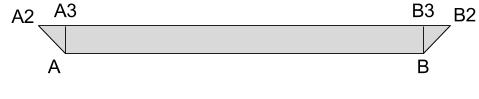
\includegraphics[width=0.75\linewidth]{Nomenclaturas_vertices_2}
    \caption{Nomenclatura final de los vértices.}
    \label{fig:nomenclatura_vertices_2}
\end{figure}

Con la nueva geometría presentada en la figura \ref{fig:nomenclatura_vertices_2} convertimos las paredes en dos prismas triangulares unidos por dos planos superior e inferior de la pared. Con esto conseguimos que los planos anterior y posterior sean totalmente idénticos aunque con las normales invertidas. Esto, sin embargo, complicará sensiblemente las conexiones entre los vértices (Fig. \ref{fig:nueva_estructura}).

\begin{figure}[H]
    \centering
    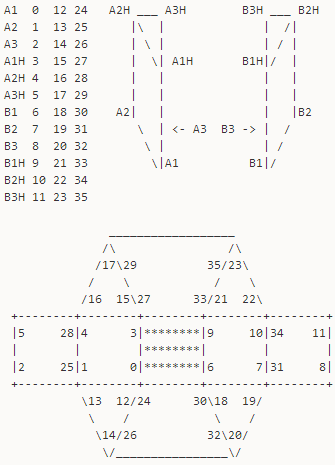
\includegraphics[scale=0.75]{Final_wall_structure}
    \caption{Estructura final de las paredes, sin incluir los planos anterior y posterior.}
    \label{fig:nueva_estructura}
\end{figure}

Con los índices:

\begin{lstlisting}
#define INDICES {\
    1,  3,  0,      1,  4,  3,  \
    2,  28, 25,     2,  5,  28, \
    14, 13, 12,     16, 17, 15, \
    26, 30, 32,     26, 24, 30, \
    27, 35, 33,     27, 29, 35, \
    6,  10, 7,      6,  9,  10, \
    31, 11, 8,      31, 34, 11, \
    20, 18, 19,     21, 23, 22, \
}
\end{lstlisting}

El resto de información se calcula exactamente del mismo modo partiendo de los nuevos vértices e índices.

%%%%%%%%%%%%%%%%%%%%%%%%%%%%%%%%%%%%%%%%%%%%%%%%%%%%%%%%%%%%%%%%%%%%%%%%%%%%%
%%%%%%%%%%%%%%%%%%%%%%%%%%%%%%%%%%%%%%%%%%%%%%%%%%%%%%%%%%%%%%%%%%%%%%%%%%%%%
%%%%%%%%%%%%%%%%%%%%%%%%%%%%%%%%%%%%%%%%%%%%%%%%%%%%%%%%%%%%%%%%%%%%%%%%%%%%%
\clearpage
\subsection{Generación de ventanas I: proyección sobre pared}
Como ya se ha mencionado en el apartado \ref{subsec:gen2}, las ventanas están definidas por un punto, una altura y un ancho. Como podemos ver no se incluye ninguna información respecto a que pared es la que va a contener dicha ventana; lo que haremos será coger la pared más cercana al punto dado.

Para ello proyectaremos el punto sobre la línea $AB$ de cada una de las paredes, y calcularemos la distacia hasta cada una de las proyecciones para ver cuál es la más cercana (véase el apéndice \ref{sec:pointrayproj} sobre la proyección punto-línea):

\begin{lstlisting}
unsigned int WallManager::findWall(glm::vec3 point) {
	unsigned int nearest = (unsigned int)-1;
	float nearest_distance = -1.f, distance;
	
	for (unsigned int i = 0; i < n_walls; ++i) {
		glm::vec3 projection;
		if (Utils::point_line_projection(
		        (*wall_list[i])[LogicPlane::A1], 
		        (*wall_list[i])[LogicPlane::B1], 
		        point, 
		        projection
		    )) {
			
			distance = glm::length(projection - point);
			if ( nearest_distance < 0.f || 
			     distance < nearest_distance
			   ) {
				nearest_distance = distance;
				nearest = i;
			}
		}
	}
	return nearest;
}
\end{lstlisting}

Todas las ventanas o puertas han de ser necesariamente rectangulares. Esta es una precondición que se ha impuesto desde desarrollo para simplificar el cálculo de los agujeros, dado que es más sencillo incorporar geometrías más complejas inclyendo paredes falsas dentro del modelo de la ventana o puerta. Por ejemplo, si en algún momento quisiéramos incorporar una ventana redonda, sería más sencillo incluir 4 esquinas de pared a la ventana permitiendo que el agujero sea rectangular igualmente.

Como preparación para el próximo apartado (\ref{sec:wallgeowindows}) calculamos sobre la pared los 4 puntos que delimitarán la ventana sobre la pared. Para ello proyectamos el punto de la pared sobre el plano que forma esta, y calculamos el resto de puntos desplazándonos por dicho plano (véase el apéndice \ref{sec:pointplaneproj} sobre la proyección punto-rectángulo):

\begin{lstlisting}
void WindowGenerator::projectVertices(WallData& wall, WallData::Window& window) {
	glm::vec3 plane_A = wall[LogicPlane::A1];
	glm::vec3 plane_B = wall[LogicPlane::B1];
	glm::vec3 plane_C = wall[LogicPlane::A1H];

	glm::vec3 AB_dir = glm::normalize(plane_B - plane_A);
	glm::vec3 AC_dir = glm::normalize(plane_C - plane_A);

	glm::vec3 origin = Utils::point_rec_projection(plane_A, plane_B, plane_C, window.origin);

	window[LogicPlane::A1] = origin;
	window[LogicPlane::B1] = origin + AB_dir * window.width;
	window[LogicPlane::A1H] = origin + AC_dir * window.height;
	window[LogicPlane::B1H] = window[LogicPlane::A1H] + AB_dir * window.width;
}
\end{lstlisting}

%%%%%%%%%%%%%%%%%%%%%%%%%%%%%%%%%%%%%%%%%%%%%%%%%%%%%%%%%%%%%%%%%%%%%%%%%%%%%
%%%%%%%%%%%%%%%%%%%%%%%%%%%%%%%%%%%%%%%%%%%%%%%%%%%%%%%%%%%%%%%%%%%%%%%%%%%%%
%%%%%%%%%%%%%%%%%%%%%%%%%%%%%%%%%%%%%%%%%%%%%%%%%%%%%%%%%%%%%%%%%%%%%%%%%%%%%
\subsection{@TODO-Generación de ventanas II: modificación de la geometría de la pared}
\label{sec:wallgeowindows}

%%%%%%%%%%%%%%%%%%%%%%%%%%%%%%%%%%%%%%%%%%%%%%%%%%%%%%%%%%%%%%%%%%%%%%%%%%%%%
%%%%%%%%%%%%%%%%%%%%%%%%%%%%%%%%%%%%%%%%%%%%%%%%%%%%%%%%%%%%%%%%%%%%%%%%%%%%%
%%%%%%%%%%%%%%%%%%%%%%%%%%%%%%%%%%%%%%%%%%%%%%%%%%%%%%%%%%%%%%%%%%%%%%%%%%%%%
\subsection{Generación de uvs}
Para que el motor aplique correctamente las texturas sobre las paredes, se requiere que las uvs estén a escala de mundo; es decir, se espera que dada una distancia entre dos vértices de la mima malla, sus uvs tengan la misma distancia. La mayor dificultad en este caso está en que los vértices se encuentran en espacio tridimensional, mientras que las uv son coordenadas bidimensionales de la textura que estamos mapeando. Por lo tanto, debemos de algún modo desconsiderar la orientación de la pared y centrarnos en sus superficies.

Como nuestra geometría está formada por planos perfectos, la solución encontrada ha consistido en partir siempre de la esquina inferior izquierda de cada uno de ellos. Como precondición tenemos que la esquina ``A" tiene la uv (0,0).

Por lo tanto por cada plano, necesitamos definir la uv de la esquina inferior izquierda, y los vectores hacia los cuales ``avanzan" las componentes x e y de las uv (Fig. \ref{fig:datos_uvs}).

\begin{figure}[H]
    \centering
    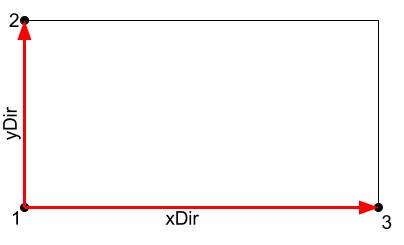
\includegraphics[scale=0.75]{Datos_uvs}
    \caption{Datos necesarios para la generación de las uv ``2" y ``3".}
    \label{fig:datos_uvs}
\end{figure}

La razón de usar proyecciones y no la magnitud de los vectores directamente, es que no sabemos en cual de las dos direcciones se encuentra el vértice que estamos mirando mientras iteramos. Proyectando cada punto tenemos la distancia en cada una de las dos direcciones y se la sumamos a la uv del vértice ``1":

\begin{lstlisting}
glm::vec2 Utils::genUV(glm::vec3 origin, glm::vec3 xDir, glm::vec3 yDir, glm::vec3 point, glm::vec2 originValue, float length_x, float length_y) {
       glm::vec2 uv;
       uv.x = point_ray_projection(origin, xDir, point);
       uv.y = point_ray_projection(origin, yDir, point);

       if (length_x > 0.f && uv.x < 0.f)
              uv.x = length_x - uv.x;
       if (length_y > 0.f && uv.y < 0.f)
              uv.y = length_y - uv.y;

       uv = uv + originValue;
       return uv;
}
\end{lstlisting}

Dado que las uv no pueden ser negativas, se hace un paso en las líneas 6-9 para que, en caso de serlo, se les sume la longitud total del lado en el que se encuentran.

%%%%%%%%%%%%%%%%%%%%%%%%%%%%%%%%%%%%%%%%%%%%%%%%%%%%%%%%%%%%%%%%%%%%%%%%%%%%%
%%%%%%%%%%%%%%%%%%%%%%%%%%%%%%%%%%%%%%%%%%%%%%%%%%%%%%%%%%%%%%%%%%%%%%%%%%%%%
%%%%%%%%%%%%%%%%%%%%%%%%%%%%%%%%%%%%%%%%%%%%%%%%%%%%%%%%%%%%%%%%%%%%%%%%%%%%%
\subsection{Generación de normales, tangentes y bitangentes}
El cálculo de cada normal es el resultado de la suma de la normal de cada polígono en el que se encuentra dicho vértice, y para calcular esta se hace el producto vectorial (normalizado) de los vectores que van del primer vértice hacia el segundo y el tercero:

\begin{lstlisting}
// Edges of the triangle
glm::vec3 vec1 = v2 - v1;
glm::vec3 vec2 = v3 - v1;

glm::vec3 normal = glm::normalize(glm::cross(vec1, vec2));
\end{lstlisting}

Las tangentes y bitangentes son un poco más complicadas: todo vector tiene infinitos vectores tangentes, pero en este caso no nos sirve cualquiera. El vector tangente a la normal tiene que estar siempre alineado con las uv.

Como se explica en el tutorial 13 de opengl-tutorial.org, para ello debemos resolver el siguiente sistema de ecuaciones:


\[ deltaPos1 = deltaUV1.x * T + deltaUV1.y * B \]
\[ deltaPos2 = deltaUV2.x * T + deltaUV2.y * B \]

Esto se traduce en nuestro código a:

\begin{lstlisting}
// UV vectors
glm::vec2 deltaUV1 = uv2 - uv1;
glm::vec2 deltaUV2 = uv3 - uv1;

float r = 1.0f / (deltaUV1.x * deltaUV2.y - deltaUV1.y * deltaUV2.x);
glm::vec3 tangent = (vec1 * deltaUV2.y - vec2 * deltaUV1.y) * r;
glm::vec3 bitangent = (vec2 * deltaUV1.x  - vec1 * deltaUV2.x)*r;
\end{lstlisting}

Ahora que ya tenemos todos los pasos necesarios para generar paredes básicas, podemos empezar a ver los primeros resultados. A continuación podemos ver un ejemplo de habitación cerrada con el recorrido (0,0),(0,3),(3,6),(6,3),(6,0),(3,1.5) (Fig. \ref{fig:walls_test_1}).

\begin{figure}[H]
    \centering
    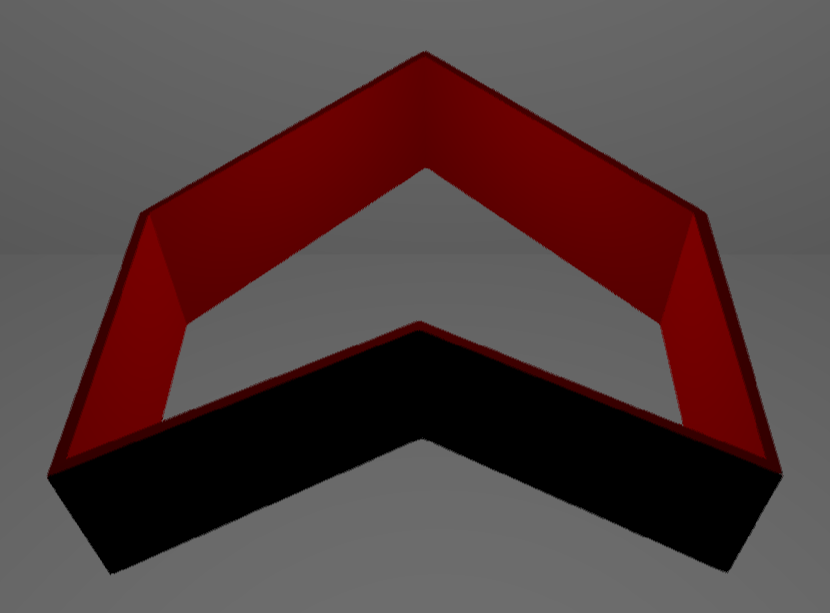
\includegraphics[width=0.7\linewidth]{Walls_test1}
    \caption{Resultado de las primeras pruebas.}
    \label{fig:walls_test_1}
\end{figure}
